\documentclass[border=0pt]{standalone}
\usepackage{pgfplots}
\pgfplotsset{width=\linewidth,compat=1.8}
\usepackage{amsmath}
\usepackage{pgfplotstable}
\usepgfplotslibrary{fillbetween}
\providecommand{\datapath}{.}

\pgfplotsset{every tick label/.append style={font=\boldmath\huge}}
\tikzstyle{every node}=[font=\bfseries\LARGE]

\begin{document}
\pgfplotstableread[col sep=comma,]{\datapath/dcfr9.csv}\dcfrb
\pgfplotstableread[col sep=comma,]{\datapath/dcfr16.csv}\dcfra
\pgfplotstableread[col sep=comma,]{\datapath/cams.csv}\cams
\LARGE
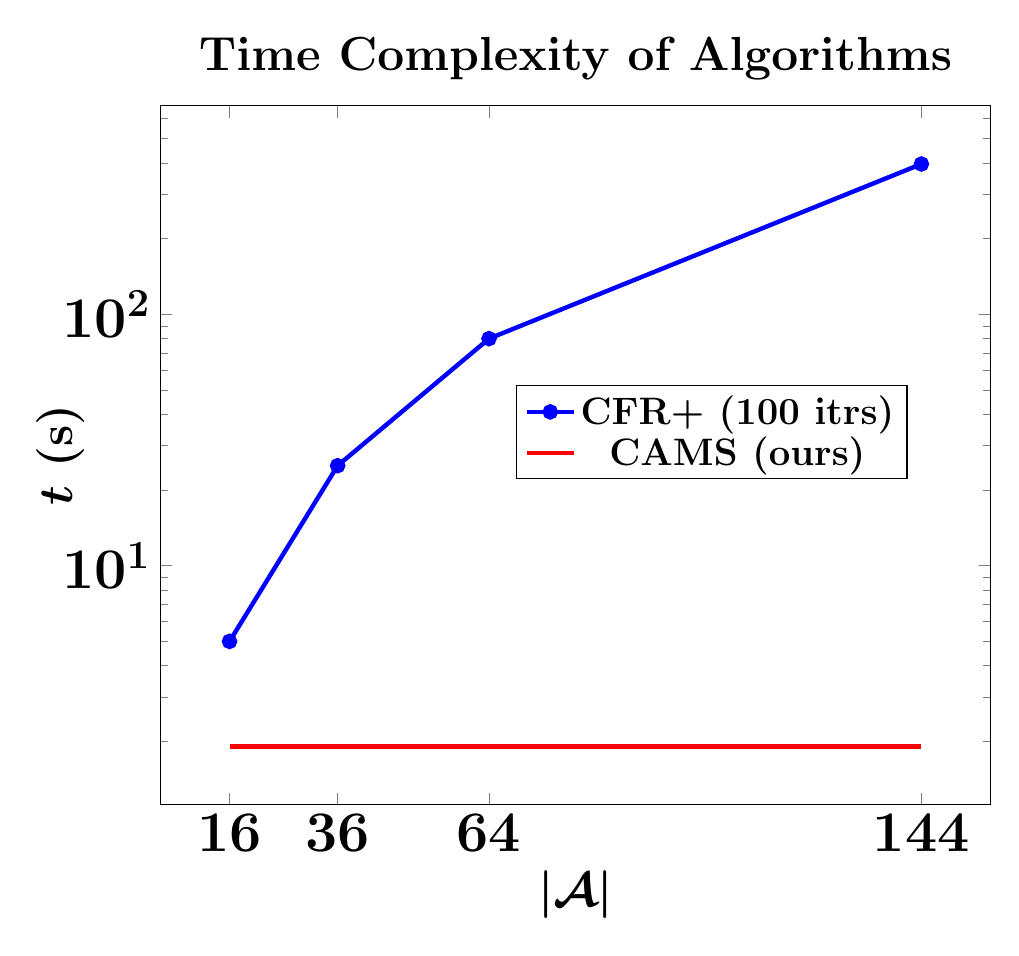
\begin{tikzpicture}[scale=1]
\begin{axis}[title={Time Complexity of Algorithms},
    legend style={nodes={scale=0.8}, style={at={(0.9, 0.6)}}},
    legend entries={CFR+ (100 itrs), CAMS (ours)},
    xlabel={$\boldsymbol{|\mathcal{A}|}$},
    ylabel={$\boldsymbol{t}$ (s)},
    xtick={16, 36, 64, 144},
    ymode=log,
    ylabel shift=-15pt,
]
\addplot [mark=*, mark size=2pt, ultra thick, blue] coordinates {
(16, 5)
(36, 25)
(64, 80)
(144, 396)
};
\addplot [ultra thick, red] coordinates {
(16, 1.91)
(36, 1.91)
(64, 1.91)
(144, 1.91)
};
\end{axis}
\end{tikzpicture}%
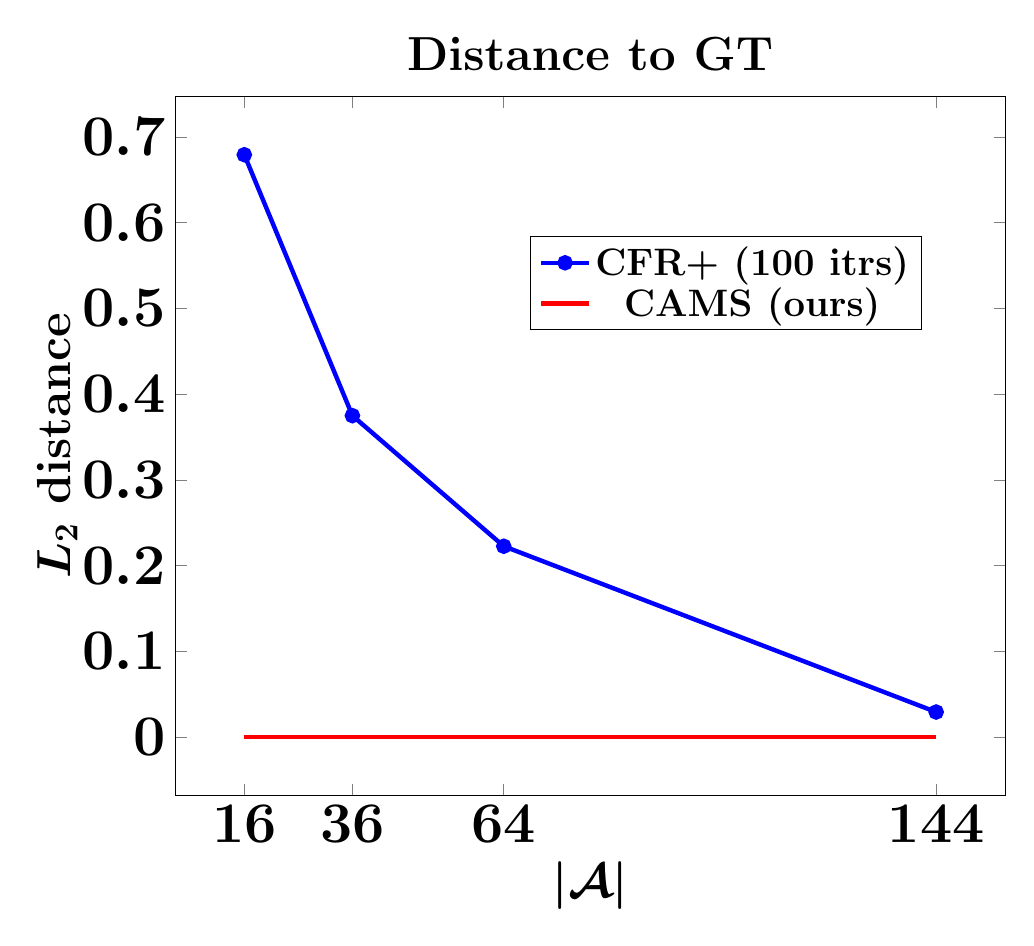
\begin{tikzpicture}[scale=1]
\begin{axis}[title={Distance to GT},
    legend style={nodes={scale=0.8}, style={at={(0.9, 0.8)}}},
    legend entries={CFR+ (100 itrs), CAMS (ours)},
    xlabel={$\boldsymbol{|\mathcal{A}|}$},
    ylabel={$\boldsymbol{L_2}$ distance},
    xtick={16, 36, 64, 144},
    % ymode=log,
    ylabel shift=-5pt,
]
\addplot [mark=*, mark size=2pt, ultra thick, blue] coordinates {
(16, 0.67932191)
(36, 0.375022)
(64, 0.2227114)
(144, 0.0293452)
};
\addplot [ultra thick, red] coordinates {
(16, 0)
(36, 0)
(64, 0)
(144, 0)
};
\end{axis}
\end{tikzpicture}%
\begin{tikzpicture}[scale=1.03]
    \begin{axis}[title={Distance to GT}, every axis title/.style={above, at={(0.5, 0.986)}},
    legend style={nodes={scale=0.8}, style={at={(0.55, 0.95)}}},
    legend entries={DeepCFR $\boldsymbol{(|\mathcal{A}|=16)}$, DeepCFR $\boldsymbol{(|\mathcal{A}|=9)}$, CAMS (ours)},
    xlabel={$\boldsymbol{t}$},
    ylabel={Mean $\boldsymbol{L_2}$ distance},
    xtick={0, 0.25, 0.5, 0.75},
    ytick={0, 5, 10, 15},
    % ymode=log,
    xmax=0.8,
    ylabel shift=-5pt,
]
% A =16
\addplot [mark=*, mark size=2pt, ultra thick, blue] table[x=x,y=y] {\dcfra};
% A =9
\addplot [mark=*, mark size=2pt, ultra thick, teal] table[x=x,y=y] {\dcfrb};
% cams
\addplot [mark=*, mark size=2pt, ultra thick, red] table[x=x,y=y] {\cams};
% fill betweens
% cfr_9
\addplot [name path=upper,draw=none] table[x=x,y expr=\thisrow{y}+\thisrow{err}] {\dcfrb};
\addplot [name path=lower,draw=none] table[x=x,y expr=\thisrow{y}-\thisrow{err}] {\dcfrb};
\addplot [fill=teal!40, fill opacity=0.4] fill between[of=upper and lower];
% cfr_16
\addplot [name path=upper_2,draw=none] table[x=x,y expr=\thisrow{y}+\thisrow{err}] {\dcfra};
\addplot [name path=lower_2,draw=none] table[x=x,y expr=\thisrow{y}-\thisrow{err}] {\dcfra};
\addplot [fill=blue!40, fill opacity=0.4] fill between[of=upper_2 and lower_2];
% cams
\addplot [name path=upper_3,draw=none] table[x=x,y expr=\thisrow{y}+\thisrow{err}] {\cams};
\addplot [name path=lower_3,draw=none] table[x=x,y expr=\thisrow{y}-\thisrow{err}] {\cams};
\addplot [fill=red!10] fill between[of=upper_3 and lower_3];
\end{axis}
\end{tikzpicture}
\end{document}